\documentclass[11pt]{article}
\usepackage[a4paper,margin=2.5cm]{geometry}
\usepackage{amsmath,amssymb}
\usepackage[T1]{fontenc}
\usepackage{lmodern}
\usepackage{graphicx}
\usepackage{booktabs}
\usepackage{array}
\usepackage{algorithm}
\usepackage{algorithmic}
\usepackage{tikz}
\usepackage[section]{placeins}
% Online Resource layout: captions in the journal's style (small type, label then a quad, caption above tables
% with a gap to the top rule), supplement numbering S1, S2, ... so no table or figure shares a number with the
% main paper, and more room between floats and the surrounding text
\usepackage[font=small,labelfont=bf,labelsep=quad,skip=6pt]{caption}
\captionsetup[table]{position=top}
\captionsetup[figure]{name=Fig.}
\renewcommand{\thetable}{S\arabic{table}}
\renewcommand{\thefigure}{S\arabic{figure}}
\setlength{\intextsep}{16pt plus 4pt minus 2pt}
\setlength{\textfloatsep}{18pt plus 4pt minus 2pt}
\setlength{\floatsep}{16pt plus 4pt minus 2pt}
\usetikzlibrary{arrows.meta,fit,shapes.symbols,shapes.geometric,positioning,calc}
\title{Online Resource 1\\[4pt]\large Supplementary material for the article ``AXIOM: A Shared Graph-Attention Controller for Scalable Multi-Agent 5G Slice Admission''\\[2pt]\normalsize Wireless Personal Communications}
\author{Manoj Prasad Kunasegran, Wai Leong Pang, Swee King Phang\\[4pt]
\small Corresponding author Wai Leong Pang, \texttt{waileong.pang@taylors.edu.my}\\
\small School of Engineering, Faculty of Innovation and Technology, Taylor's University,\\
\small 47500 Subang Jaya, Selangor, Malaysia}
\date{}
\begin{document}
\maketitle

\section*{S1. Overview}
This supplement gives the detail behind the main paper's verification runs and additional results. Every pass criterion was fixed in a pre-registration committed before the run it judged, and every check is reported whether it held or failed. The baselines are a single-agent deep Q-network (DQN-SA), independent per-gNB deep Q-networks (DQN-I), and multi-agent proximal policy optimisation (MAPPO), where DQN denotes a deep Q-network in general. AXIOM's encoder is a graph attention network (GAT), and its variant with a per-node multi-layer perceptron (MLP) encoder is called the MLP variant. Table~\ref{tab:s-acronyms} lists the other acronyms used in this supplement.

\begin{table}[!htbp]
\caption{Acronyms used in this supplement}
\label{tab:s-acronyms}
\centering
\footnotesize
\begin{tabular}{@{}l>{\raggedright\arraybackslash}p{0.36\textwidth}@{\hspace{1.5em}}l>{\raggedright\arraybackslash}p{0.36\textwidth}@{}}
\toprule
Acronym & Meaning & Acronym & Meaning \\
\midrule
CI & Confidence interval & PRB & Physical resource block \\
DP & Differential privacy & RAN & Radio access network \\
DP-SGD & Differentially private stochastic gradient descent & RF & Radio frequency \\
eMBB & enhanced Mobile Broadband & RIC & RAN Intelligent Controller \\
FedAvg & Federated averaging & SDR & Software-defined radio \\
gNB & gNodeB, the 5G base station & SLA & Service Level Agreement \\
mMTC & massive Machine-Type Communication & TDD & Time-division duplex \\
OAI & OpenAirInterface & UDP & User Datagram Protocol \\
O-RAN & Open Radio Access Network & UE & User equipment \\
& & URLLC & Ultra-Reliable Low-Latency Communication \\
\bottomrule
\end{tabular}
\end{table}

\section*{S2. Verification runs}
We reran eleven reported settings on their original seeds in fresh processes, and each reproduced its stored per-seed results exactly, as did the Env A oracle rule on all 30 seeds. DQN-SA is the one exception, because its training code builds the network before it sets the seed. Five reruns of one affected seed earned 7.45 to 9.67 reward per step, against 8.74 stored. Dropping the affected seeds changes no comparison's direction. AXIOM's lead in Env A at three gNBs moves from $+0.311$ to $+0.241$ per step but now passes the Holm correction, at $p=0.039$ against 0.066.

Four further runs retrained every policy on seeds from 3000 onwards, never used before. The first used 20 seeds at three gNBs, 15 in Env A at nineteen gNBs, and 10 in Env B at seven gNBs. All 26 predictions stated in advance for these fresh seeds held. In Env A AXIOM reached 98.2\% of the oracle reward at three gNBs and at nineteen gNBs kept 95.6\% priority-slice compliance against 47.8\% to 65.5\% for the baselines. In Env B the tuned local rule again beat it, earning 9.175 against 8.782 per step. Two results were less favourable to AXIOM than the main campaigns. In Env A at three gNBs AXIOM won 11 of 20 seeds against DQN-SA but trailed it by 0.021 per step on average, at $p=0.07$. In Env B at seven gNBs the MLP variant beat graph attention by 1.38 reward per step, in 9 of 10 seeds at $p=0.006$.

The second run covered Env A at seven and nineteen gNBs and federated training, on ten seeds each. At nineteen gNBs AXIOM kept 96.5\% priority-slice compliance against 47.5\% to 65.2\% for the baselines, and federation again showed no significant cost, at $+0.077$ with 95\% CI [$-$1.03, 1.27]. At seven gNBs AXIOM kept 96.7\% priority-slice compliance and led every baseline under both layouts. Under the fully-connected layout, however, two weak AXIOM seeds at 57.2\% and 76.9\% left its leads of 12.5 to 25.3 points short of significance after Holm correction. DQN-I and DQN-SA also reached 80.9\% and 80.6\% compliance, above the 80\% bound we had set, so three of the eleven checks in this run failed.

The third run covered every remaining claim, and 43 of its 48 checks held. At seven gNBs on the hex layout and at nineteen on the fully-connected layout AXIOM kept 99.0\% and 95.7\% priority-slice compliance and beat every baseline. A twenty-seed rerun of the seven-gNB fully-connected layout then held all six tests at Holm-adjusted $p\leq0.007$. Three of the five failures concern the baselines rather than AXIOM. On fresh seeds at seven gNBs DQN-I and DQN-SA kept 76.2\% to 83.3\% priority-slice compliance, above the 80\% bound in three settings. The other two come from the load study. At 102\% load two weak AXIOM seeds left it at 96.8\% of the oracle reward, a gap that is not significant at $p=0.25$, and below DQN-SA's mean, at 12.551 against 12.910. Every dropout and churn cost was significant at Holm-adjusted $p\leq0.041$, no gap between AXIOM and a baseline survived correction, and AXIOM kept a spike block precision of 0.97. Per-step privacy noise lowered reward by 0.65 to 1.31 per step, with no drop surviving correction. In Env B the original AXIOM again earned less than the current design in all ten seeds, by 2.19 per step. With its initialisation seeded, DQN-SA then reproduced exactly across processes. AXIOM's lead over it in Env A at three gNBs becomes $+0.254$ per step at Holm-adjusted $p=0.018$, and $+0.948$ on the replication seeds. In Env B the lead stays at $+1.320$, and at nineteen gNBs the seeded baseline collapses in 28 of 30 seeds and trails AXIOM by 32.3 points.

The fourth run enlarged the two unstable samples, and four of its five checks held. On 40 new seeds in Env A at three gNBs AXIOM reached 98.1\% of the oracle, tying it in 27 seeds, but its lead over the seeded DQN-SA was only $+0.159$ per step, at $p=0.090$. On 20 new seeds at 102\% load the seeded DQN-SA again earned slightly more, 12.978 against 12.945 per step.

An independent script with its own log reader and Holm correction recomputes every results table and key sentence of both documents from the raw logs, and all of its checks pass. Fresh seeds therefore confirmed the main findings of the paper. At seven and nineteen gNBs in Env A AXIOM kept 93.4\% to 100\% priority-slice compliance and beat every baseline under every layout. The exceptions are a small and unstable lead over DQN-SA in Env A at three gNBs and baseline compliance of up to 83\% at seven gNBs. AXIOM's small lead over DQN-SA in Env A at three gNBs did not recur, at margins of $-0.021$ and $0.159$ reward per step on 20 and 40 new seeds. In one ten-seed load sample two weak AXIOM seeds also left it 3.2\% short of the oracle, a gap that a twenty-seed rerun did not reproduce.

Fig.~\ref{fig:s-forest} sets each reported comparison with a learned baseline beside its fresh-seed counterpart. Of the 38 reported differences whose 95\% CI excludes zero, 35 keep a CI on the same side on fresh seeds. The three exceptions all concern cluster-level compliance in Env B. AXIOM's deficits of 9.2 points to DQN-SA and 4.8 points to DQN-I at seven gNBs become 4.2 points and a 0.8-point lead. Its lead over MAPPO at nineteen gNBs falls to 2.9 points, and all three fresh CIs span zero.

\begin{figure}[!htbp]
\centering
\includegraphics[width=0.85\textwidth]{figures/fig_forest.pdf}
\caption{AXIOM minus each learned baseline, with 95\% CIs. Solid lines and filled circles are the reported runs, dashed lines and hollow diamonds the fresh seeds. a, Reward per gNB. b, Cluster-level priority-slice compliance}
\label{fig:s-forest}
\end{figure}

\section*{S3. Live testbed and deployment check}
\begin{figure}[!htbp]
\centering
\resizebox{\textwidth}{!}{%
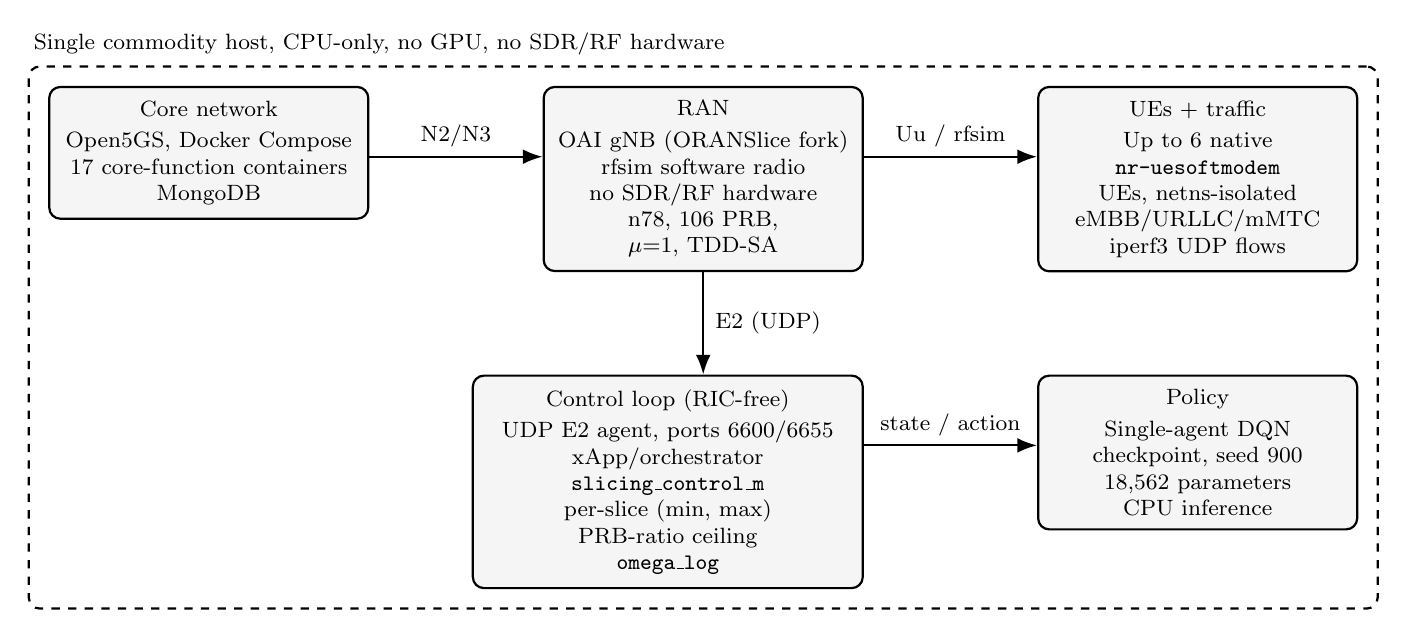
\begin{tikzpicture}[
  block/.style={draw, thick, rounded corners, align=center, fill=gray!8,
                font=\footnotesize, inner sep=5pt, text width=3.7cm},
  arr/.style={-{Latex[length=2.5mm]}, thick},
  lbl/.style={font=\footnotesize, inner sep=1pt}
]
\node[block, anchor=north] (core) at (0,0)
  {Core network\\[2pt]
   Open5GS, Docker Compose\\
   17 core-function containers\\
   MongoDB};
\node[block, anchor=north west] (ran) at ($(core.north east)+(2.2,0)$)
  {RAN\\[2pt]
   OAI gNB (ORANSlice fork)\\
   rfsim software radio\\
   no SDR/RF hardware\\
   n78, 106 PRB, $\mu{=}1$, TDD-SA};
\node[block, anchor=north west] (ues) at ($(ran.north east)+(2.2,0)$)
  {UEs + traffic\\[2pt]
   Up to 6 native \texttt{nr-uesoftmodem} UEs, netns-isolated\\
   eMBB/URLLC/mMTC iperf3 UDP flows};
\node[block, anchor=north east, text width=4.6cm] (ctrl) at ($(ran.south east)+(0,-1.3)$)
  {Control loop (RIC-free)\\[2pt]
   UDP E2 agent, ports 6600/6655\\
   xApp/orchestrator \texttt{slicing\_control\_m}\\
   per-slice (min, max) PRB-ratio ceiling\\
   \texttt{omega\_log}};
\node[block, anchor=north] (policy) at (ues.south |- ctrl.north)
  {Policy\\[2pt]
   Single-agent DQN checkpoint, seed 900\\
   18{,}562 parameters\\
   CPU inference};
\draw[arr] ($(core.north east)+(0,-0.9)$) -- ($(ran.north west)+(0,-0.9)$) node[lbl, midway, above=2pt] {N2/N3};
\draw[arr] ($(ran.north east)+(0,-0.9)$) -- ($(ues.north west)+(0,-0.9)$) node[lbl, midway, above=2pt] {Uu / rfsim};
\draw[arr] (ran.south) -- (ran.south |- ctrl.north) node[lbl, midway, right=3pt] {E2 (UDP)};
\draw[arr] ($(ctrl.north east)+(0,-0.9)$) -- ($(policy.north west)+(0,-0.9)$) node[lbl, midway, above=2pt] {state / action};
\node[draw, thick, dashed, rounded corners, inner sep=7pt, fit=(core)(ran)(ues)(ctrl)(policy)] (host) {};
\node[font=\footnotesize, anchor=south west, inner sep=2pt] at ($(host.north west)+(0,0.05)$)
  {Single commodity host, CPU-only, no GPU, no SDR/RF hardware};
\end{tikzpicture}%
}
\caption{Real testbed stack, a single-host, software-radio rfsim,
RIC-free O-RAN deployment distinguished from software-defined-radio hardware-in-the-loop
testbeds. Every block and label is a measured or configured value from
this rig}
\label{fig:testbed}
\end{figure}

Every live measurement comes from the single-host, software-radio O-RAN stack of Fig.~\ref{fig:testbed}. It runs without a near-real-time RAN Intelligent Controller (RIC), because the ORANSlice fork applies slicing control directly through a lightweight User Datagram Protocol (UDP) E2 agent. AXIOM itself is not deployed on the live testbed. Its multi-gNB policy needs at least two live gNBs, and our two-gNB attempt registered both with the core but did not sustain traffic. The testbed therefore validates the pipeline AXIOM would use, namely the E2 control path, PRB-ratio actuation, and real-time inference. It does so with a single-agent DQN checkpoint trained offline for this rig, at one and at two User Equipments (UEs) per slice.

A capacity probe showed every slice served at essentially 100\% of offered demand with 0.000\% loss. The checkpoint's real accept and reject decisions, typically blocking mMTC alone, ran correctly through the E2 loop. Because the rig never ran short of capacity, this shows that the pipeline works, not admission under contention. A scheduler-configuration error that granted fewer PRBs than the gNB scheduler's five-PRB floor was fixed at the root. Instrumentation then confirmed zero below-floor grants across more than 100{,}000 readings.

\section*{S4. Additional setup details}
Fig.~\ref{fig:overview} gives an overview of the research, and Table~\ref{tab:params} lists the simulation and training parameters shared by both environments. Algorithm 1 of the main paper states AXIOM's training loop.

\begin{figure}[!htbp]
\centering
\resizebox{0.98\textwidth}{!}{%
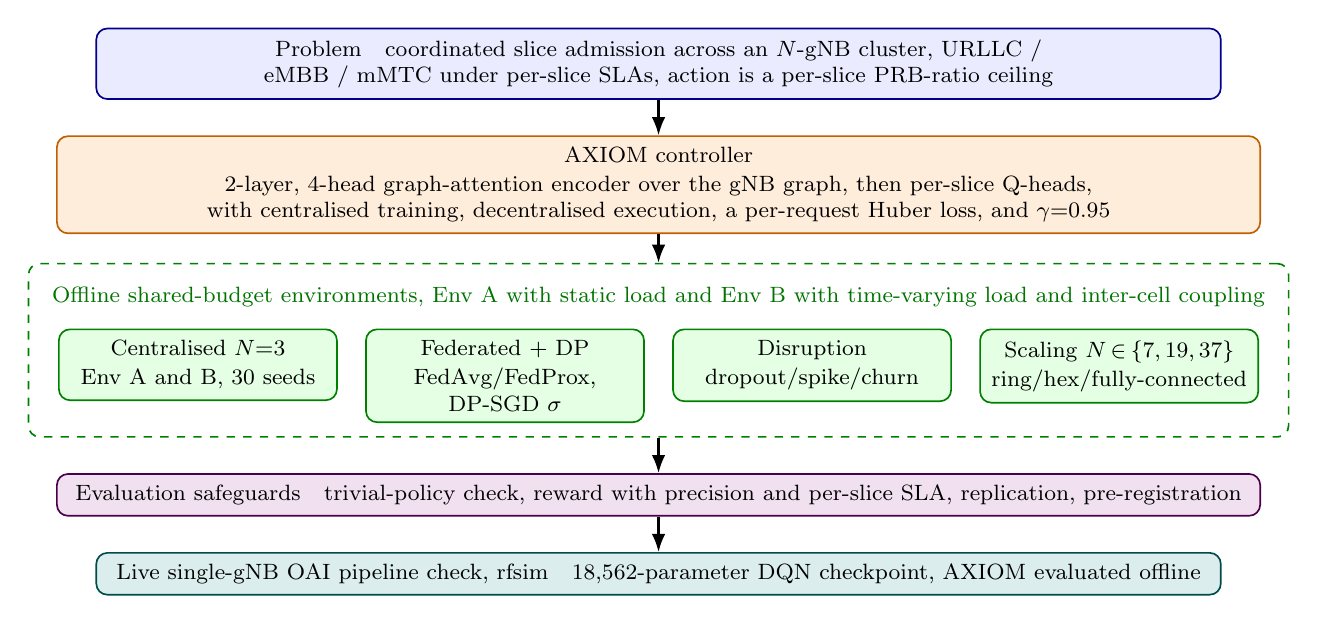
\begin{tikzpicture}[
  base/.style={draw, semithick, rounded corners, align=center, font=\footnotesize, inner sep=4pt},
  pblk/.style={base, fill=blue!8,   draw=blue!55!black},
  ablk/.style={base, fill=orange!14, draw=orange!75!black},
  cblk/.style={base, fill=green!10,  draw=green!50!black, text width=3.25cm, anchor=north},
  sblk/.style={base, fill=violet!12, draw=violet!60!black},
  lblk/.style={base, fill=teal!14,   draw=teal!60!black},
  ar/.style={-{Latex[length=2.3mm]}, thick}
]
\node[pblk, text width=14cm] (prob) at (8,7.4)
  {Problem\quad coordinated slice admission across an $N$-gNB cluster, URLLC / eMBB / mMTC under per-slice SLAs, action is a per-slice PRB-ratio ceiling};
\node[ablk, text width=15cm, below=0.45cm of prob] (arch)
  {AXIOM controller\\[1pt] 2-layer, 4-head graph-attention encoder over the gNB graph, then per-slice Q-heads, with centralised training, decentralised execution, a per-request Huber loss, and $\gamma{=}0.95$};
\node[font=\footnotesize, text=green!45!black, anchor=north] (glab) at ($(arch.south)+(0,-0.55)$)
  {Offline shared-budget environments, Env A with static load and Env B with time-varying load and inter-cell coupling};
\node[cblk] (c1) at ($(glab.south)+(-5.85,-0.15)$) {Centralised $N{=}3$\\[1pt] Env A and B, 30 seeds};
\node[cblk] (c2) at ($(glab.south)+(-1.95,-0.15)$) {Federated + DP\\[1pt] FedAvg/FedProx, DP-SGD $\sigma$};
\node[cblk] (c3) at ($(glab.south)+(1.95,-0.15)$) {Disruption\\[1pt] dropout/spike/churn};
\node[cblk] (c4) at ($(glab.south)+(5.85,-0.15)$) {Scaling $N\!\in\!\{7,19,37\}$\\[1pt] ring/hex/fully-connected};
\node[draw=green!50!black, semithick, rounded corners, dashed, inner sep=5pt, fit=(glab)(c1)(c2)(c3)(c4)] (grp) {};
\node[sblk, text width=15cm, below=0.45cm of grp] (safe)
  {Evaluation safeguards\quad trivial-policy check, reward with precision and per-slice SLA, replication, pre-registration};
\node[lblk, text width=14cm, below=0.45cm of safe] (live)
  {Live single-gNB OAI pipeline check, rfsim\quad 18{,}562-parameter DQN checkpoint, AXIOM evaluated offline};
\draw[ar] (prob) -- (arch);
\draw[ar] (arch) -- (grp.north);
\draw[ar] (grp.south) -- (safe);
\draw[ar] (safe) -- (live);
\end{tikzpicture}%
}
\caption{Overview of the research. An AXIOM controller is evaluated
across four offline campaigns in two shared-budget environments, every result
checked by evaluation safeguards, with the deployment pipeline checked on a live single-gNB testbed}
\label{fig:overview}
\end{figure}

\begin{table}[!htbp]
\caption{Simulation and training parameters, shared by both environments unless stated}
\label{tab:params}
\centering
\footnotesize
{\setlength{\tabcolsep}{3pt}
\begin{tabular}{@{}>{\raggedright\arraybackslash}p{0.36\textwidth} >{\raggedright\arraybackslash}p{0.58\textwidth}@{}}
\toprule
Parameter & Value \\
\midrule
PRB budget per gNB, $B$ & 100 \\
Nominal share, floor, cap, in PRB ratio & URLLC 30, 5, 33\newline eMBB 60, 10, 66\newline mMTC 10, 5, 11 \\
Priority weight $\omega_k$ & URLLC 12.0, eMBB 3.5, mMTC 0.3 \\
Per-accept reward $R_k$ & 1.0 for every slice \\
Violation penalty $\lambda_k$ & URLLC 10.0, eMBB 5.0, mMTC 2.5 \\
Latency and loss budgets & URLLC 15 ms, 0.8\%\newline eMBB 45 ms, 2.0\%\newline mMTC 65 ms, 3.5\% \\
Congestion coefficient $\kappa$, load-balance weight $\beta$ & 1.5, 1.0 \\
Episode & 60 steps of 5 s, with queues emptied at each episode start \\
Requests per step & $N$, each with a uniformly random slice and gNB, with at most $4N$ pending \\
Offered demand per slice & 105\% of nominal share, per-step noise $0.005B$, per-gNB multiplier in $[0.9, 1.0]$ \\
Env B load and coupling & $0.95\,(1+0.3\sin(2\pi(s+\psi_i)/60))$, $B_i(t)=B\,(1-0.15\,\bar u_{\mathcal{N}(i)}(t-1))$ \\
Admission gate step & 5 PRB-ratio points per accept or reject \\
Training and evaluation & 300 and 50 episodes per seed, held-out evaluation stream \\
Value-based learners & Adam, learning rate $10^{-3}$, $\gamma=0.95$, $\epsilon$ from 1.0 to 0.05 at $\times0.985$ per episode, replay 10,000, minibatch 16, warm-up 32, target sync every 10 episodes \\
AXIOM network & Two-layer, four-head GAT, hidden and output 16, raw-feature skip, per-slice Q-heads of hidden 32, Huber loss, gradient clip 1.0 \\
DQN baselines & Two hidden layers of 128, squared-error loss \\
MAPPO & Actor and critic learning rate $10^{-3}$, 10 epochs, minibatch 64, clip 0.2, entropy 0.01, generalised advantage estimation $\lambda=0.95$ \\
\bottomrule
\end{tabular}}
\end{table}

A sensitivity study repeats the learned policies and the oracle rule in Env A on 10 seeds at 102\% and 107\% of the nominal load and with changed slice weights, eMBB lowered from 3.5 to 2.5 and mMTC raised from 0.3 to 0.6. A second repeats AXIOM in Env B on 10 seeds at learning rates of $3{\times}10^{-4}$ and $3{\times}10^{-3}$ and with an encoder twice as wide. The federated campaign runs in Env A on seeds 900 to 909, with noise multipliers $\sigma \in \{0, 0.5, 1, 2, 4\}$ and a replication on seeds 1000 to 1009. Each round runs 50 local steps of federated averaging (FedAvg) with a gradient-clip norm of $1.0$.

A validation screen checks every trained checkpoint of every learned policy before evaluation. Each plays five greedy episodes on its own training stream and fails if it blocks no request or if fewer than 90\% of its blocks target mMTC. Every seed is reported whether or not it passes. In Env B the reward-optimal policy also sheds eMBB, so an amendment recorded before any result was read makes the no-blocking criterion the primary screen there. The two Env B constants were calibrated on pilot seeds with rules only. The main pre-registration fixed them together with AXIOM's learning rate and skip connection, all chosen on pilot seeds 2000 to 2009.

AXIOM's encoder is a graph-attention network over the gNB graph. At every control step each gNB forms its own feature row $\mathbf{x}_i$ of PRB-used ratio, congestion level, and normalised queue length. A two-layer network with $H{=}4$ heads then produces one embedding per gNB. Each head $h$ uses a learned source vector $\mathbf{a}_s^{h}$ and destination vector $\mathbf{a}_d^{h}$ on the shared projection $\mathbf{W}^{h}$. Here $\mathrm{LeakyReLU}$ has slope $0.2$, and $\mathcal{N}_i$ is the set of neighbours of node $i$,
\begin{equation}
\label{eq:gat}
\varepsilon_{ij}^{h}=\mathrm{LeakyReLU}\big(\mathbf{a}_s^{h\top} \mathbf{W}^{h} \mathbf{x}_i + \mathbf{a}_d^{h\top} \mathbf{W}^{h} \mathbf{x}_j\big),
\qquad
\alpha_{ij}^{h}=\frac{\exp\varepsilon_{ij}^{h}}{\sum_{l\in\mathcal{N}_i}\exp\varepsilon_{il}^{h}}.
\end{equation}
Here $\varepsilon_{ij}^{h}$ is the unnormalised attention score from node $i$ to neighbour $j$ in head $h$, and $\alpha_{ij}^{h}$ is its normalisation over $i$'s neighbours, with $l$ ranging over $\mathcal{N}_i$. Hidden layers concatenate the $H$ heads under an exponential linear unit (ELU), while the final layer averages them. A per-layer normalisation $\mathrm{LN}(\cdot)$ then rescales each node's embedding to zero mean and unit variance, giving the per-gNB embedding $\mathbf{z}_i$,
\begin{equation}
\label{eq:gat-agg}
\mathbf{z}_i=\mathrm{LN}\!\Big(\tfrac{1}{H}\textstyle\sum_{h=1}^{H}\sum_{j\in\mathcal{N}_i}\alpha_{ij}^{h}\,\mathbf{W}^{h} \mathbf{x}_j\Big).
\end{equation}
Every agent's loss updates this shared encoder, so training sees the full cluster state. At execution each agent reads only its own row $\mathbf{z}_i$ to decide its pending requests. An earlier variant mixed each gNB's summed per-request values with a QMIX-style monotonic mixer. Its target changed scale with the request count, and its mean training loss diverged from about 76 to about 409. Treating each request as its own sample removed that dependence.

In the federated variant each client's encoder still reads the full joint node-feature snapshot. Differential privacy bounds how much any one client's training data can change what the shared model reveals. Each client applies a differentially private stochastic gradient descent (DP-SGD) step, clipping its minibatch gradient to norm $C_{\text{dp}}$ and adding Gaussian noise of standard deviation $\sigma C_{\text{dp}}$. Zero-concentrated differential privacy (zCDP) composes this over the $m$ noisy steps a client takes, with $\varepsilon$ and $\delta$ the usual privacy-loss and failure-probability parameters,
\begin{equation}
\label{eq:zcdp}
\rho=\frac{2m}{\sigma^{2}},\qquad
\varepsilon(\delta)=\rho+2\sqrt{\rho\ln(1/\delta)}.
\end{equation}
We credit no amplification by subsampling, because minibatches come from a replay buffer that reuses records, so the bound is conservative. The noise protects each client's admission decisions and rewards, but not the congestion features that every encoder reads by design.

An AI assistant, Anthropic's Claude, was used to help write the analysis and plotting scripts and to edit the manuscript text. The authors made all research decisions and take full responsibility for the content of this paper.

\section*{S5. Evaluation safeguard details}
The trivial-policy check evaluates the simplest rules before trusting any learned policy. In our first simulator every slice was served independently against its own ceiling. There, accepting every request earned 14.45 reward per step and kept URLLC and eMBB at 100\% SLA compliance, more than any learned policy, so admission control had nothing to do. The shared-budget simulator of the main paper removes that loophole. Over the same 30 held-out seeds, accepting every request now earns 9.89 reward per step and lets eMBB compliance fall to 56.8\%, whereas shedding every mMTC request earns 12.84 and keeps URLLC and eMBB at 100\%.

Replication on a disjoint seed sample caught one artefact. Queue backlog carried over between episodes, so one early transient spoiled every later episode for every policy, the oracle rule included. Every result in this paper comes from the corrected simulator, which empties all queues at the start of each episode.

\section*{S6. Additional results}
In the nineteen-gNB hex cluster AXIOM keeps the URLLC and eMBB gates at 1.00 and 0.97, while closing the mMTC gate to 0.08. DQN-SA leaves every gate open at 0.99 and DQN-I closes the mMTC gate only to 0.92. MAPPO partly closes the eMBB gate to 0.82 but leaves mMTC open at 0.69. In the thirty-seven-gNB cluster of the main paper DQN-SA leaves every gate open at 0.93 to 0.95 and DQN-I closes the mMTC gate only to 0.94. MAPPO there partly closes the eMBB gate to 0.80 but leaves mMTC open at 0.51.

The MLP variant reads only a gNB's own features, and Table~\ref{tab:s-mlp} sets it beside AXIOM at three gNBs. In Env A it ties AXIOM, which earns 0.058 more reward per step at three gNBs with 95\% CI [$-$0.17, 0.26] and 0.31 more at nineteen gNBs on the ring layout, with 7 of 12 seeds tied. In Env B it earns slightly more, 0.116 per step at three gNBs in 17 of 30 seeds at $p=0.45$. At seven gNBs it earns 1.12 and 0.95 more, but neither lead survives Holm correction. It uses 3,190 parameters at every cluster size and takes 0.77, 1.69, 4.46, and 9.44 ms per control step at 3, 7, 19, and 37 gNBs. Its median training time is 503 s per seed in Env B at three gNBs.

\begin{table}[!htbp]
\caption{AXIOM and its MLP variant at three gNBs, 30 seeds per policy, 95\% bootstrap CIs. Columns as in the main paper's three-gNB tables}
\label{tab:s-mlp}
\centering
\footnotesize
\begin{tabular}{@{}lccccc@{}}
\toprule
Env A & Reward/step & Precision & Collapsed & URLLC & eMBB \\
\midrule
AXIOM & 12.698 [12.49, 12.86] & 0.992 & 0/30 & 0.998 & 0.979 \\
AXIOM, MLP encoder & 12.640 [12.46, 12.79] & 0.986 & 0/30 & 1.000 & 0.976 \\
\midrule
Env B & Reward/step & URLLC & eMBB & mMTC \\
\midrule
AXIOM & 8.832 [8.64, 9.03] & 0.958 & 0.344 & 0.406 \\
AXIOM, MLP encoder & 8.948 [8.77, 9.13] & 0.974 & 0.337 & 0.452 \\
\bottomrule
\end{tabular}
\end{table}

A disjoint replication on seeds 1000 to 1009 is stronger for AXIOM. There it earns 1.083, 0.799, and 3.806 more reward per step than DQN-SA, DQN-I, and MAPPO. It sits only 0.018 below the oracle on those seeds. Pooled over all 40 seeds its margins over the three baselines are 0.504, 1.032, and 2.965 reward per step at Holm-adjusted $p\leq0.002$. It falls 0.108 short of the oracle, a small gap that is significant at $p=0.034$. Fresh seeds in Section S2 do not reproduce the lead over DQN-SA, however. In Env B at three gNBs the disjoint ten-seed replication points the same way, with AXIOM winning 7 or 8 of 10 seeds against each, but no lead survives correction there.

Under 102\% and 107\% load and the changed slice weights AXIOM stays within 0.13 of the oracle rule's reward. Fig.~\ref{fig:m2-results} shows the per-seed evidence at three gNBs. Its leads over both DQN baselines are positive under every condition, but at ten seeds only two survive correction. They are its margin over DQN-I at 107\% load, 1.073 reward per step at $p=0.006$, and over DQN-SA under the changed weights, 1.264 at $p=0.041$.

The comparison also holds when the baselines are made stronger. A grid of 24 MAPPO configurations, chosen on pilot seeds and allowing three times the training budget, kept the reported setting in Env B and selected a longer-trained one in Env A. There MAPPO rises from 10.013 to 11.448 reward per step at three gNBs and from 60.6\% to 69.6\% priority-slice compliance at nineteen gNBs on the ring layout. AXIOM still beats it in every setting tested, by 1.25 to 16.18 reward per step at Holm-adjusted $p<0.001$, and by 2.42 in Env B at seven gNBs. With its initialisation properly seeded, DQN-SA keeps 80.3\% and 63.9\% priority-slice compliance at seven and nineteen gNBs, and AXIOM beats it under every layout at Holm-adjusted $p\leq0.035$.

\begin{figure}[!htbp]
\centering
\includegraphics[width=\textwidth]{figures/fig3_m2_results.pdf}
\caption{Env A, three gNBs, per-seed evidence. a, Paired per-seed mean reward
per step of AXIOM versus DQN-SA, coloured by win, tie, or loss.
b, Per-seed reward distribution for AXIOM and the two DQN baselines}
\label{fig:m2-results}
\end{figure}

AXIOM's learning rate matters most as the cluster grows. The original AXIOM, at $10^{-4}$, came slightly closer to the oracle in Env A, tying it in 39 of 40 seeds. In Env B it earns only 6.496 per step on seeds 900 to 909, and $3{\times}10^{-4}$ reaches 7.220. The DQN baselines also lose reward when rerun at $10^{-4}$, falling to 11.477 [10.61, 12.09] and 11.119 [10.73, 11.50] reward per step in Env A at three gNBs, with 95\% CIs. A rate of $3{\times}10^{-3}$ and an encoder twice as wide both stay within 0.19 of the current AXIOM. At nineteen gNBs in Env A the original AXIOM kept priority-slice compliance at only 79.1\%. Over the Env B seeds the original AXIOM earns 2.37 less per step than the current design in all ten seeds.

\begin{figure}[!htbp]
\centering
\includegraphics[width=\textwidth]{figures/fig4_m3_privacy.pdf}
\caption{Federated campaign in Env A, 10 seeds. a, Paired per-seed federation
cost on mean reward per step, not significant at $p=0.65$. b, Block precision
versus DP noise multiplier $\sigma$, over the seeds that block}
\label{fig:m3-privacy}
\end{figure}

Fig.~\ref{fig:m3-privacy} shows the federated campaign in Env A on ten seeds. With federation and no noise, mean reward per step on the ten shared seeds is 12.356 for centralised AXIOM and 11.929 for the federated variant. That is a difference of $+0.427$ with 95\% CI [$-$0.54, 1.51] and $p=0.65$, so federation shows no significant cost on these seeds. The disjoint replication shows a larger cost of $+0.968$, with 95\% CI [0.18, 1.96], which falls just short of significance at $p=0.055$. FedProx on three seeds gives no consistent picture, with $\mu{=}0.01$ above FedAvg and $\mu$ of 0.1 and 1.0 below it.

DP-SGD noise on every step lowers reward by 0.77 to 1.25 per step at every tested noise multiplier. It also lowers eMBB compliance to between 74.3\% and 83.0\%, and two and four of the ten seeds collapse at $\sigma$ of 2 and 4. None of these drops survives Holm correction at ten seeds. Each client takes 17{,}969 noisy steps over its training run. At $\delta{=}10^{-5}$ Eq.~\eqref{eq:zcdp} then gives $\varepsilon$ of about 146{,}000, 37{,}000, 9{,}600, and 2{,}600 for $\sigma$ of 0.5, 1, 2, and 4. Per-step DP-SGD therefore gives no meaningful guarantee here. A useful one would need noise on the roughly 360 per-round model updates instead.

Each policy's frozen Env A checkpoint also faced three disruptions at evaluation time. A gNB dropout forces one gNB to reject everything and blanks its feature row. A demand spike multiplies the arrival rate, and an agent churn swaps one gNB's decisions for an untrained copy of its policy. Dropout and churn windows last 10\%, 30\%, or 60\% of the episode. Spikes multiply arrivals by 2, 4, or 8. Reward is normalised by each step's pending-request count, and Fig.~\ref{fig:m4-disruption} plots the reward each policy keeps.

\begin{figure}[!htbp]
\centering
\includegraphics[width=\textwidth]{figures/fig5_m4_disruption.pdf}
\caption{Disruption campaign, 10 seeds per policy, 95\% CIs. a, b, Normalised
reward kept under dropout and churn, with the undisrupted level at the tick marked None.
c, Block precision under demand spikes}
\label{fig:m4-disruption}
\end{figure}

Dropout and churn hurt every policy significantly at every severity, in 9 or 10 of 10 seeds at Holm-adjusted $p\leq0.041$, and no gap between AXIOM and any baseline survives correction. Under the two longer churn windows AXIOM keeps less reward than DQN-I, 1.88 and 1.10 against 2.29 and 1.72, though not significantly. Demand spikes leave AXIOM's decisions largely intact, with block precision at 0.98, against 1.00 for DQN-SA and about 0.95 for DQN-I. A disjoint replication on seeds 1000 to 1009 reproduces this pattern, with every dropout and churn cost significant at $p\leq0.035$ and no significant gap between policies.

The validation screen rarely rejects AXIOM in Env A. It fails 1 of 30 seeds at three gNBs, 1 of 45 at seven, and 5 of 90 at nineteen. At thirty-seven gNBs it fails 8 of AXIOM's 60 checkpoints, all six collapsed ones among them. It fails 29, 27, and 27 of 30 for DQN-SA, DQN-I, and MAPPO. In Env B no learned policy collapsed at three or seven gNBs, while at nineteen gNBs DQN-SA collapsed in 14 of 15 seeds and AXIOM in 1, as Section S10 lists.

\begin{figure}[!htbp]
\centering
\includegraphics[width=\textwidth]{figures/fig12_training_curves.pdf}
\caption{Training curves, mean step reward per training episode over 12 seeds with
95\% bands, smoothed over 10 episodes. a, b, Env B at three and seven gNBs.
c, Env A at 19 gNBs on the ring layout}
\label{fig:curves}
\end{figure}

In training, shown in Fig.~\ref{fig:curves}, MAPPO rises fastest early but plateaus lowest in every panel. The value-based learners rise more slowly but further. At nineteen gNBs AXIOM keeps improving to about 85 per step over the last 20 training episodes, while the two DQN baselines settle near 71 and 74. AXIOM's slowest decision takes 0.2\% of the 5 s control period, so its inference cost does not constrain deployment. Fig.~\ref{fig:s-layouts} gives the per-layout view of the Env A scaling results that the main paper pools over layouts.

\begin{figure}[!htbp]
\centering
\includegraphics[width=\textwidth]{figures/fig14_layouts.pdf}
\caption{Env A priority-slice compliance by layout, per-seed points behind the mean and 95\% CI. a, Nineteen gNBs, 30 seeds per layout. b, Thirty-seven gNBs, where the baselines never read the layout and ran once, on the hex seeds}
\label{fig:s-layouts}
\end{figure}

\section*{S7. Analysis plans and development notes}
Each analysis plan was committed to the project's version-control history before the runs it governs, with one exception. The main campaign reuses Env A results of DQN-SA, DQN-I, and the oracle rule from an earlier rerun, M63. They cover three gNBs on the primary and replication seeds, the sensitivity study, seven gNBs, and 15 of the 30 seeds at nineteen gNBs. The M63 plan was committed one minute after that rerun was launched and before any of its results were read. Two development stages are also disclosed, although neither changed a reported result. A protocol, M67, tried to make AXIOM beat both DQN baselines decisively in Env A at three gNBs. Checkpoint selection brought AXIOM to the oracle but brought DQN-SA within 0.05 of it too. A test of both encoders on ten new seeds in Env B at seven gNBs then found no significant lead over DQN-SA, so AXIOM was not changed. Exploratory probes on seeds 900 to 904 and pilot seeds 2000 to 2004 suggested the load-shift effect of Section S8 and the hindsight bound of the main paper's Env B results before their reported runs. Three figures describe stored runs after the results were known, with no plan or test of their own. The main paper maps per-gNB compliance at nineteen gNBs. Section S2 sets reported beside fresh-seed differences, and Section S13 shows AXIOM's learned eMBB shedding after replaying every stored evaluation exactly.

\section*{S8. Shifted load, longer training, and the joint target on fresh seeds}
No deployable policy we tested keeps eMBB compliance above 37\% in Env B, because demand at the load peaks exceeds the budget by up to 23.5\%. Even the rule with the highest eMBB compliance among all 95 local rules, chosen in hindsight on each evaluation stream, reaches only 37.7\% on average. The best rule by reward in hindsight earns only 0.14\% more than the tuned rule.

Table~\ref{tab:s-shift} lists AXIOM against the rule tuned on nominal conditions, on 25 checkpoints neither retrained nor re-tuned. A rule re-tuned on the shifted training streams selected thresholds different from the nominal rule's at every shift. Against it AXIOM trails by 0.16 and 0.12 per step at 110\% and 115\% load, which is not significant, and by 0.62 at 120\% load. Under 110\% to 120\% load AXIOM beats the nominally tuned rule in 21 to 23 of 25 seeds at Holm-adjusted $p\leq0.0002$. At seven gNBs on the ring layout the reversal is larger. AXIOM trails the rule by 3.84 reward per step under nominal load but leads it by 1.86 and 3.14 at 110\% and 120\% load. Under lighter load or stronger coupling the tuned rule keeps a lead that is not significant.

\begin{table}[!htbp]
\caption{AXIOM against the rule tuned on nominal conditions, Env B with three gNBs, 25 seeds, reward per step, wins over losses, and the unadjusted Wilcoxon $p$}
\label{tab:s-shift}
\centering
\begin{tabular}{lccccc}
\toprule
Condition & AXIOM & Tuned rule & Difference & AXIOM wins & $p$ \\
\midrule
80\% load & 13.776 & 14.055 & $-$0.279 & 12/13 & 0.44 \\
nominal & 8.846 & 9.261 & $-$0.415 & 7/18 & 0.00016 \\
105\% load & 4.482 & 4.183 & +0.299 & 21/4 & 0.017 \\
110\% load & 2.082 & 1.624 & +0.458 & 23/2 & 8.8e-05 \\
115\% load & 0.378 & $-$0.052 & +0.431 & 23/2 & 1e-05 \\
120\% load & $-$0.714 & $-$1.068 & +0.354 & 21/4 & 8.8e-05 \\
coupling 0.30 & 6.457 & 6.766 & $-$0.310 & 11/14 & 0.28 \\
load swing 0.50 & 6.015 & 5.831 & +0.184 & 18/7 & 0.045 \\
\bottomrule
\end{tabular}
\end{table}

With three times the training budget AXIOM gains 0.33 reward per step at three gNBs and 2.92 at seven, on 20 and 12 seeds. The remaining gaps to the tuned rule, 0.08 and 0.96 per step, are no longer significant, at $p=0.35$ and $p=0.064$. The joint-target variant of AXIOM, trained beside it on fresh seeds, never differed significantly from it after Holm correction over eight tests. It reaches 12.831 reward per step in Env A at three gNBs and 99.96\% priority-slice compliance at nineteen. On 60 further fresh seeds across four settings it was again never significantly different from AXIOM, ahead in three settings and behind at seven gNBs in Env B, so we keep the reported design.

\section*{S9. Cluster-size scaling and thirty-seven gNBs}
At seven gNBs AXIOM keeps URLLC and eMBB at 99.8\% and 94.4\%, against 91.4\% and 61.0\% for DQN-SA, 94.2\% and 55.0\% for DQN-I, and 87.0\% and 48.4\% for MAPPO. At nineteen gNBs it keeps them at 99.4\% and 95.1\%, and at thirty-seven at 96.7\% and 90.7\%. AXIOM's priority-slice compliance stays between 97.1\% and 98.9\% from three to nineteen gNBs while every baseline falls. Its lead over the best baseline grows to 32.0 points at nineteen gNBs, with a parameter count that does not change. DQN-I ignores the layout and gives identical results under all three, which checks that the layout changes nothing else.

The thirty-seven-gNB configuration extends the nineteen-gNB one exactly as the seven- and nineteen-gNB configurations extended three, with 37 arrivals per step and at most 148 pending requests. No hyperparameter was tuned for this size, and each gNB sees 1.15 pending requests per step on average, as at every other size. A wrapper extends the framework's hex layout to a third ring and reproduces its seven- and nineteen-cell layouts exactly. AXIOM ran 30 seeds on the hex layout and 15 on each of the ring and fully-connected layouts. In Env A the baselines and the static rule never read the layout, so each ran once on the 30 hex seeds, and Table~\ref{tab:s-n37} lists every policy.

\begin{table}[!htbp]
\caption{Env A with thirty-seven gNBs. Priority-slice compliance is the mean of URLLC and eMBB compliance, and collapse counts policies that accept every request}
\label{tab:s-n37}
\centering
\begin{tabular}{lcccccc}
\toprule
Policy & Runs & URLLC & eMBB & Priority SLA & Reward & Collapsed \\
\midrule
AXIOM, hex & 30 & 97.4\% & 89.8\% & 93.6\% & 174.20 & 3 \\
AXIOM, ring & 15 & 93.7\% & 92.6\% & 93.2\% & 173.51 & 2 \\
AXIOM, fully-connected & 15 & 98.4\% & 90.4\% & 94.4\% & 174.44 & 1 \\
DQN-SA & 30 & 73.3\% & 44.1\% & 58.7\% & 144.70 & 26 \\
DQN-I & 30 & 38.6\% & 25.7\% & 32.1\% & 148.35 & 3 \\
MAPPO & 30 & 67.8\% & 45.6\% & 56.7\% & 145.25 & 0 \\
Static rule & 30 & 100.0\% & 100.0\% & 99.98\% & 177.58 & 0 \\
\bottomrule
\end{tabular}
\end{table}

AXIOM's six collapsed runs are seeds 918, 919, and 924 on the hex layout, 901 and 1001 on the ring, and 902 on the fully-connected layout. They keep 59\% to 65\% priority-slice compliance, while its other runs keep 96.9\% to 98.1\% on average under each layout. We also ran MAPPO with the configuration that the main paper's grid selected for Env A, trained for 900 episodes. It keeps 65.6\% priority-slice compliance and 151.90 reward per step and never collapses. AXIOM beats it by 29.2 points in 13 of 15 seeds at $p<0.001$ and by 23.23 reward per step in all 15.

The fresh-seed replication retrained every policy on seeds 6100 to 6119 on the hex layout, as Table~\ref{tab:s-n37-fresh} lists. AXIOM leads DQN-SA by 37.7 points of priority-slice compliance and 35.46 reward per step, DQN-I by 61.0 and 25.62, and MAPPO by 36.5 and 30.63. It wins 18 to 19 of 20 seeds in every comparison, all at Holm-adjusted $p<0.001$. Its one collapsed seed is 6110, and pooled with the 30 hex seeds above, AXIOM keeps 94.2\% priority-slice compliance over 50 seeds and collapses in 4 of them.

\begin{table}[!htbp]
\caption{Env A with thirty-seven gNBs on 20 fresh seeds, hex layout}
\label{tab:s-n37-fresh}
\centering
\begin{tabular}{lcccccc}
\toprule
Policy & Seeds & URLLC & eMBB & Priority SLA & Reward & Collapsed \\
\midrule
AXIOM & 20 & 95.4\% & 94.7\% & 95.1\% & 174.67 & 1 \\
DQN-SA & 20 & 71.6\% & 43.1\% & 57.4\% & 139.20 & 18 \\
DQN-I & 20 & 42.0\% & 26.1\% & 34.1\% & 149.04 & 2 \\
MAPPO & 20 & 70.1\% & 47.0\% & 58.5\% & 144.04 & 0 \\
Static rule & 20 & 100.0\% & 100.0\% & 99.97\% & 177.68 & 0 \\
\bottomrule
\end{tabular}
\end{table}

\section*{S10. Accept-all at scale, tuned DQN baselines, and Env B at nineteen gNBs}
Accepting every request is the floor that any admission controller should clear. In Env A it keeps 70.9\%, 67.1\%, and 61.9\% priority-slice compliance at seven, nineteen, and thirty-seven gNBs. Its reward there is 26.88, 78.55, and 156.22 per step. At seven gNBs only MAPPO, at 67.7\%, falls below it. At nineteen and thirty-seven gNBs every baseline does, and DQN-SA's runs that do not collapse keep only 40.0\% and 35.9\%, DQN-I's 55.9\% and 29.1\%. AXIOM keeps 97.1\%, 97.3\%, and 93.7\% at the same three sizes.

The DQN baselines were tuned on pilot seeds over learning rates from $10^{-4}$ to $10^{-3}$ and minibatches of 16 and 64, and retrained on the 30 hex seeds wherever a new setting won, as Table~\ref{tab:s-tuned} lists. The grid selected new settings in three of the four combinations of baseline and size. No tuned baseline exceeds the accept-all floor at either size. Several DQN-SA settings tie on the pilot seeds because they collapse into accept-all there, and at nineteen gNBs the selected setting won by 0.001 reward per step. It then accepts every request in all 30 evaluation seeds. AXIOM beats each tuned baseline on compliance and reward in every setting, winning 26 to 30 of 30 seeds at Holm-adjusted $p<0.001$.

\begin{table}[!htbp]
\caption{DQN baselines tuned on pilot seeds, Env A, 30 hex seeds. LR is the learning rate, batch the minibatch size, and Before the priority-slice compliance before tuning}
\label{tab:s-tuned}
\centering
\small
\setlength{\tabcolsep}{4pt}
\begin{tabular}{lcccccc}
\toprule
Baseline & gNBs & LR, batch & Priority SLA & Before & Reward & Collapsed \\
\midrule
DQN-SA & 19 & $10^{-4}$, 16 & 67.1\% & 65.3\% & 78.55 & 30 \\
DQN-I & 19 & $3{\times}10^{-4}$, 64 & 59.1\% & 56.4\% & 77.07 & 11 \\
DQN-SA & 37 & $10^{-3}$, 16, unchanged & 58.7\% & 58.7\% & 144.70 & 26 \\
DQN-I & 37 & $10^{-4}$, 64 & 45.5\% & 32.1\% & 150.42 & 18 \\
\bottomrule
\end{tabular}
\end{table}

Table~\ref{tab:s-envb19} lists Env B at nineteen gNBs on the hex layout, over 15 seeds. Per-gNB compliance counts a slice as compliant at a gNB and step when that gNB meets the slice's SLA, whereas the cluster-level metric counts a violation at any gNB as a violation of the cluster. AXIOM makes exactly the static rule's decisions in 9 of the 15 seeds, and in 5 of the other 6 it also blocks only mMTC.

\begin{table}[!htbp]
\caption{Env B with nineteen gNBs, 15 seeds, hex layout. SLA columns give priority-slice compliance, the mean of URLLC and eMBB compliance, per gNB and at cluster level}
\label{tab:s-envb19}
\centering
\small
\begin{tabular}{lcccc}
\toprule
Policy & Reward & Per-gNB SLA & Cluster SLA & Collapsed \\
\midrule
AXIOM & 80.28 & 77.3\% & 24.7\% & 1 \\
DQN-SA & 74.74 & 66.4\% & 18.0\% & 14 \\
DQN-I & 71.20 & 66.8\% & 16.7\% & 0 \\
MAPPO & 59.07 & 71.8\% & 20.8\% & 0 \\
Static rule & 81.59 & 79.9\% & 23.0\% & 0 \\
Accept all & 74.77 & 66.4\% & 18.0\% & 15 \\
Tuned local rule, carried over & 84.09 & 84.5\% & 55.7\% & 0 \\
\bottomrule
\end{tabular}
\end{table}

\section*{S11. Fifth-review runs}
This section lists every policy in the runs that answer the fifth internal review, in Tables~\ref{tab:s-vdn} to~\ref{tab:s-pergnbpen}. Four of its six predictions failed, and every result is reported. The value-decomposition network (VDN) trains DQN-I's per-gNB networks on one joint target per step, with no tuning. The per-gNB penalty charges each slice's violation penalty once for every violating gNB, in training and evaluation. Under uneven load each gNB's load multiplier is drawn between 75\% and 125\% per seed, and the rule re-tuned on those streams sheds eMBB once the URLLC queue passes 0.05 rather than 0.2.

VDN ties AXIOM at three gNBs in both environments but falls behind at nineteen gNBs, as Table~\ref{tab:s-vdn} shows. There AXIOM keeps 13.6 percentage points more and earns 2.73 more reward per step, winning 27 to 28 of 30 seeds at Holm-adjusted $p<0.001$. At 110\% and 120\% of the nominal load at nineteen gNBs, AXIOM keeps 24.3 to 34.0 and 2.5 to 6.4 percentage points more priority-slice compliance than every learned baseline, at Holm-adjusted $p\leq0.006$, as Table~\ref{tab:s-oversub} lists. At 120\% the priority demand exceeds the slice caps at most gNBs, so no policy can protect it throughout.

In Env B at nineteen gNBs under raised load the carried-over tuned rule keeps more per-gNB compliance than AXIOM by shedding eMBB. Meanwhile the static rule earns 1.8 to 2.0 more reward than AXIOM, which makes the static rule's decisions in 9 to 11 of the 15 seeds. When per-gNB load differs widely instead, with multipliers drawn between 75\% and 125\% at seven gNBs, AXIOM does not beat the nominally tuned rule, earning 0.36 more reward per step at $p=0.23$. It ties a rule re-tuned to these conditions, while the static rule earns 0.27 more at $p=0.028$. It still beats every learned baseline there, by 1.18 to 4.28 reward per step at unadjusted $p\leq0.005$. Against MAPPO under uneven per-gNB load at seven gNBs it earns 27\% more and wins every seed. Under nominal load at seven gNBs it earns between 7\% and 15\% more, significantly on two of the three layouts. Charging the SLA penalty per violating gNB, so that it grows with the cluster, raised AXIOM's per-gNB compliance by only 1.9 points, at $p=0.65$. AXIOM still did not beat the static rule. Under that reward every learned baseline kept 13.7 to 18.5 percentage points less per-gNB compliance than AXIOM, in every seed.

\begin{table}[!htbp]
\caption{VDN against AXIOM and DQN-I, reward per step and priority-slice compliance, 30 seeds per cell}
\label{tab:s-vdn}
\centering
\small
\setlength{\tabcolsep}{3pt}
\begin{tabular}{lcccccc}
\toprule
Cell & VDN & AXIOM & DQN-I & VDN SLA & AXIOM SLA & DQN-I SLA \\
\midrule
Env A, 3 gNBs & 12.664 & 12.698 & 11.587 & 99.0\% & 98.9\% & 92.9\% \\
Env B, 3 gNBs & 8.552 & 8.832 & 7.794 & 62.5\% & 65.1\% & 59.0\% \\
Env A, 19 gNBs, hex & 86.428 & 89.161 & 76.388 & 83.4\% & 97.0\% & 56.4\% \\
\bottomrule
\end{tabular}
\end{table}

\begin{table}[!htbp]
\caption{Env A with nineteen gNBs on the hex layout under higher offered load, 15 seeds. SLA is priority-slice compliance}
\label{tab:s-oversub}
\centering
\small
\setlength{\tabcolsep}{3pt}
\begin{tabular}{lcccccc}
\toprule
Policy & Reward, 110\% & SLA, 110\% & Collapsed & Reward, 120\% & SLA, 120\% & Collapsed \\
\midrule
AXIOM & 84.58 & 63.4\% & 0 & 77.44 & 21.7\% & 0 \\
DQN-SA & 72.81 & 34.3\% & 15 & 65.75 & 17.1\% & 14 \\
DQN-I & 71.36 & 29.5\% & 0 & 68.88 & 15.3\% & 0 \\
MAPPO & 63.72 & 39.1\% & 0 & 61.50 & 19.2\% & 0 \\
Static rule & 85.40 & 65.5\% & 0 & 77.93 & 21.9\% & 0 \\
Accept all & 72.81 & 34.3\% & 15 & 69.25 & 17.6\% & 15 \\
\bottomrule
\end{tabular}
\end{table}

\begin{table}[!htbp]
\caption{Env B with nineteen gNBs under raised load, 15 checkpoints, neither retrained nor re-tuned. Reward per step and per-gNB priority-slice compliance}
\label{tab:s-shift19}
\centering
\small
\setlength{\tabcolsep}{3pt}
\begin{tabular}{lcccccc}
\toprule
Load & AXIOM & Tuned rule & Static rule & AXIOM SLA & Tuned SLA & Static SLA \\
\midrule
Nominal & 80.28 & 84.09 & 81.59 & 77.3\% & 84.5\% & 79.9\% \\
110\% & 77.01 & 70.79 & 78.84 & 41.6\% & 56.7\% & 41.6\% \\
115\% & 76.59 & 69.04 & 78.50 & 33.4\% & 46.7\% & 33.1\% \\
120\% & 76.30 & 67.64 & 78.27 & 26.8\% & 38.5\% & 26.4\% \\
\bottomrule
\end{tabular}
\end{table}

\begin{table}[!htbp]
\caption{Env B with seven gNBs on the ring layout under uneven per-gNB load, 15 seeds. SLA is per-gNB priority-slice compliance}
\label{tab:s-hetero}
\centering
\small
\begin{tabular}{lccc}
\toprule
Policy & Reward & SLA & Collapsed \\
\midrule
AXIOM & 20.22 & 63.4\% & 0 \\
DQN-SA & 19.04 & 62.3\% & 0 \\
DQN-I & 18.65 & 61.0\% & 0 \\
MAPPO & 15.95 & 59.0\% & 0 \\
Static rule & 20.49 & 64.0\% & 0 \\
Accept all & 18.03 & 56.9\% & 15 \\
Tuned rule, carried over & 19.86 & 71.6\% & 0 \\
Tuned rule, re-tuned & 20.17 & 71.8\% & 0 \\
\bottomrule
\end{tabular}
\end{table}

\begin{table}[!htbp]
\caption{Env B with nineteen gNBs on the hex layout with the per-gNB SLA penalty, 15 seeds. Reward is under that penalty, and SLA is per-gNB priority-slice compliance}
\label{tab:s-pergnbpen}
\centering
\small
\begin{tabular}{lccc}
\toprule
Policy & Reward & SLA & Collapsed \\
\midrule
AXIOM & 23.48 & 79.2\% & 0 \\
DQN-SA & -8.69 & 65.5\% & 10 \\
DQN-I & -20.59 & 63.8\% & 0 \\
MAPPO & -45.64 & 60.6\% & 0 \\
Static rule & 23.59 & 79.9\% & 0 \\
Accept all & -0.28 & 66.4\% & 15 \\
Tuned rule, carried over & 39.41 & 84.5\% & 0 \\
\bottomrule
\end{tabular}
\end{table}

\section*{S12. Throughput and delay}
In Env B at nineteen gNBs AXIOM's URLLC delay is below every learned baseline's but above the tuned rule's. The evaluation logs record decisions, rewards, and SLA flags but not the PRBs served or the backlog. To obtain them, the usual evaluation of every stored checkpoint and rule was re-run with a recorder on the simulator's per-step output, under a plan committed before these re-runs. Every re-run whose stored log could be compared reproduced it exactly in reward, blocks, and SLA compliance. Table~\ref{tab:s-kpi} lists throughput and delay in every setting. Accept-all in Env A, which has no stored log at these seeds, is marked unchecked. Throughput is the share of offered demand that is served. The delay is the mean backlog divided by the mean served PRBs, in control periods of 5 s, with the 95th percentile taken over steps and gNBs. It is a queueing proxy from the fluid model, not packet latency.

\begin{table}[!htbp]
\caption{Served share of offered demand and backlog delay in control periods, mean and 95th percentile, per slice}
\label{tab:s-kpi}
\centering
\footnotesize
\setlength{\tabcolsep}{2.5pt}
\begin{tabular}{lcccccc}
\toprule
Policy & URLLC served & eMBB served & URLLC delay & p95 & eMBB delay & p95 \\
\midrule
\multicolumn{7}{l}{Env A, three gNBs} \\
AXIOM & 99.8\% & 99.7\% & 0.11 & 0.66 & 0.11 & 0.47 \\
DQN-SA & 99.5\% & 99.4\% & 0.20 & 0.96 & 0.18 & 0.83 \\
DQN-I & 99.4\% & 98.5\% & 0.23 & 1.11 & 0.43 & 6.24 \\
MAPPO & 98.4\% & 90.5\% & 0.38 & 3.31 & 3.81 & 19.67 \\
Static rule & 99.8\% & 99.9\% & 0.10 & 0.59 & 0.05 & 0.31 \\
Accept all, unchecked & 97.5\% & 97.6\% & 0.80 & 3.01 & 0.76 & 2.65 \\
\midrule
\multicolumn{7}{l}{Env A, thirty-seven gNBs, hex} \\
AXIOM & 99.8\% & 99.0\% & 0.08 & 0.42 & 0.34 & 1.12 \\
DQN-SA & 94.2\% & 95.2\% & 3.61 & 16.87 & 2.09 & 14.28 \\
DQN-I & 97.7\% & 97.5\% & 0.76 & 5.23 & 0.72 & 5.49 \\
MAPPO & 96.4\% & 85.7\% & 0.58 & 5.38 & 6.28 & 35.70 \\
Static rule & 100.0\% & 100.0\% & 0.03 & 0.17 & 0.02 & 0.09 \\
Accept all, unchecked & 98.7\% & 98.8\% & 0.43 & 2.14 & 0.38 & 1.83 \\
\midrule
\multicolumn{7}{l}{Env B, three gNBs} \\
AXIOM & 98.4\% & 88.5\% & 0.65 & 2.32 & 3.18 & 19.28 \\
DQN-SA & 98.2\% & 82.1\% & 0.75 & 3.15 & 5.73 & 49.79 \\
DQN-I & 98.6\% & 82.7\% & 0.66 & 2.81 & 4.73 & 49.34 \\
MAPPO & 97.2\% & 83.5\% & 1.10 & 4.00 & 4.57 & 43.82 \\
Static rule & 96.0\% & 96.1\% & 1.59 & 5.25 & 1.57 & 5.11 \\
Tuned rule & 99.0\% & 84.8\% & 0.58 & 1.96 & 3.57 & 38.55 \\
Accept all & 92.8\% & 92.9\% & 2.59 & 7.72 & 2.58 & 7.59 \\
\midrule
\multicolumn{7}{l}{Env B, nineteen gNBs, hex} \\
AXIOM & 96.6\% & 92.6\% & 1.35 & 4.67 & 3.41 & 16.01 \\
DQN-SA & 93.8\% & 93.9\% & 2.26 & 6.99 & 2.24 & 6.82 \\
DQN-I & 94.1\% & 86.1\% & 2.17 & 9.71 & 4.17 & 72.77 \\
MAPPO & 89.2\% & 88.3\% & 2.66 & 33.84 & 2.58 & 28.13 \\
Static rule & 96.8\% & 96.9\% & 1.33 & 4.65 & 1.32 & 4.50 \\
Tuned rule, carried & 99.1\% & 87.9\% & 0.51 & 1.77 & 2.78 & 25.40 \\
Accept all & 93.8\% & 93.9\% & 2.25 & 6.97 & 2.24 & 6.82 \\
\bottomrule
\end{tabular}
\end{table}

\section*{S13. Seven-gNB convergence, further reruns, and fresh seeds at nineteen gNBs}
Two further runs explain AXIOM's position in Env B at seven gNBs and recheck other results, and every one of their checks held. At seven gNBs the tuned rules earn 26.5 to 27.3 per step and beat AXIOM in all 15 seeds under every layout, while AXIOM earns 23.4 to 23.6, no more than the static rule's 23.6. At seven gNBs 28 of AXIOM's 45 seeds shed only mMTC, which is the static rule's policy. None of AXIOM's 30 seeds does this at three gNBs. Neither does any of the 45 DQN-SA or DQN-I seeds at seven, against 13 of 45 for the MLP variant. At this size AXIOM's only significant leads over a learned baseline are over MAPPO's reward. The reward charges each slice's SLA penalty once for the cluster when any gNB violates it, so shedding eMBB at one gNB pays only when the other gNBs also comply. Three reruns of the original setting reproduced it exactly.

Table~\ref{tab:s-conv} lists three changes, each tested on the ring layout with 15 seeds. Compared with the original setting, the per-gNB SLA penalty raised AXIOM's compliance by 10.7 points, a learning rate of 0.003 by 14.9, and 900 training episodes by 21.7. The Holm-adjusted $p$ values are 0.007, 0.007, and 0.0004. The per-gNB penalty changes the reward itself, so only compliance compares there. Under that reward AXIOM keeps 20.9 points more than DQN-SA trained the same way, which collapses in 11 of 15 seeds.

\begin{table}[!htbp]
\caption{Env B, seven gNBs, ring layout, 15 seeds, reward per gNB per step, priority-slice compliance, and seeds that shed only mMTC}
\label{tab:s-conv}
\centering
\footnotesize
\begin{tabular}{lccc}
\toprule
Policy & Reward per gNB & Priority SLA & mMTC-only seeds \\
\midrule
AXIOM, 300 episodes, as reported & 3.36 & 34.0\% & 11 \\
AXIOM, per-gNB SLA penalty & -- & 44.7\% & 0 \\
AXIOM, learning rate 0.003 & 3.50 & 48.9\% & 3 \\
AXIOM, 900 episodes & 3.79 & 55.7\% & 1 \\
DQN-SA, 900 episodes & 3.35 & 41.9\% & 1 \\
DQN-I, 900 episodes & 3.29 & 42.9\% & 0 \\
MAPPO, 900 episodes & 2.97 & 40.5\% & 0 \\
Tuned local rule & 3.91 & 60.5\% & 0 \\
\bottomrule
\end{tabular}
\end{table}

With 900 episodes for every learner, AXIOM keeps 12.8 to 15.2 points more compliance and earns 0.44 to 0.82 more reward per gNB than each baseline, at Holm-adjusted $p\leq0.0012$. The baselines gain at most 7.0 points from the longer budget. The tuned rule still keeps more compliance than AXIOM in all 15 seeds. DQN-SA with a seeded initialisation keeps 6.7 points less than the reported unseeded run at 300 episodes, at $p=0.048$. At nineteen gNBs the longer budget does not help. After 900 episodes seven of eight seeds still shed only mMTC, against all eight after 300.

Fig.~\ref{fig:s-decision} shows what AXIOM learned at seven gNBs on the ring layout. After 300 episodes the eMBB head of 11 of its 15 seeds would reject at no step, and pooled over all 15 it rejects on 2.0\% of gNB-steps. After 900 episodes 14 of 15 seeds reject more often as the gNB's own URLLC queue grows. Pooled, the share rises from 12.2\% below a queue of 0.05 to 71.8\% between 0.75 and 1.0, a softer form of the tuned rule's step at 0.2.

\begin{figure}[!htbp]
\centering
\includegraphics[width=0.85\textwidth]{figures/fig_decision.pdf}
\caption{What AXIOM learned in Env B at seven gNBs on the ring layout, 15 seeds. a, Share of gNB-steps on which its eMBB head would reject, by the gNB's own URLLC queue, with 95\% CIs over seeds. b, How often each queue level occurs}
\label{fig:s-decision}
\end{figure}

Sixteen runs that no earlier rerun covered matched their stored per-seed results exactly, in Env A at seven, nineteen, and thirty-seven gNBs and in Env B at seven gNBs. On 15 fresh seeds, 7000 to 7014, in Env B at nineteen gNBs the results of Section S10 held again. AXIOM earned 5.90 to 22.00 more reward per step than each learned baseline and kept 6.9 to 11.1 points more per-gNB priority-slice compliance, at Holm-adjusted $p\leq0.011$, keeping 76.9\%. The static rule again earned more, by 0.87 per step, and tied AXIOM exactly in 13 of the 15 seeds. The local rule carried over from seven gNBs won every seed, by 3.33 per step, and DQN-SA collapsed in all 15.

\end{document}
